\documentclass[a4paper,10pt]{article}
\usepackage[margin=3cm, nohead]{geometry}
\usepackage{natbib}
\usepackage{graphicx}
\usepackage{listings}
\usepackage{synttree}
\usepackage{algorithm}
\usepackage{algorithmic}
\usepackage{subfig}

\newcommand{\HRule}{\rule{\linewidth}{0.5mm}}

\begin{document}

\begin{titlepage}
\begin{center}

\includegraphics[width=1\textwidth]{uva}\\[1cm]

\HRule \\[0.4cm]
{ \huge \bfseries Tweedejaarsproject A.E.S.I.}\\[0.4cm]

\HRule \\[1cm]

\textsc{\LARGE  Artificial Evolution and Swarm Intelligence}\\[0.5cm]
\textsc{\Large  Verslag}\\[1cm]

\begin{tabular*}{0.95\textwidth}{@{\extracolsep{\fill}} l c r}
Jeroen \textsc{Rooijmans}	& Maarten \textsc{Inja}     & Maarten \textsc{de Waard} \\
\textsc{5887410}                &\textsc{5872464}           &\textsc{5894883}\\
\end{tabular*}

\vfill \today
\end{center}
\end{titlepage}
\tableofcontents \pagebreak

\section{Introduction}
During this project we will attempt to create a program that artificially evolves tank like agents in the RoboCode environment\footnote{RoboCode home page: http://robocode.sourceforge.net/}.
RoboCode is a simple game, where virtual tanks can fight eachother. More information and rules of the game can be found in section \ref{bi}.\\

It would be fairly easy to write a powerful bot ourselves, but using genetic programming\footnote{Genetic Programming wiki: http://en.wikipedia.org/wiki/Genetic\_programming} we can let a computer evolve these bots.
To test our evolved bots, we use the RoboCode environment to generate test data of battles between our evolved bots and various enemy bots. After a certain amount of battles, RoboCode generates results, these results consist of a overall score. The score is calculated using the survival rate, damage done and ranking of the previously fought battles.

There is a similar program that evolves RoboCode bots created by Klaus Meffert, the program is called RoboCode with JGAP\footnote{RoboCode with JGAP home page: http://jgap.sourceforge.net/doc/robocode/robocode.html}. After short research we found out that this program is implemented different from ours. It does not evolve on the code, like we want to, but it enables code segments, making evolving to a good bot a lot easier.

Bots we use as enemies can be bots that come with RoboCode, self written bots or bots that won online tournaments, informations and rankings of these tournaments can be found on RoboRumble\footnote{RoboRumble home page: http://robowiki.net/wiki/RoboRumble}.
The code for this project will be written in Java and available on our Google Code page \footnote{Google Code page: http://code.google.com/p/aesi/}.
We planned our activities with the Gantt chart that can be found in Appendix \ref{planning}.

\section{Project goals}
The main goal of this project is to create a Java program that evolves RoboCode bots.
These bots will evolve based on their performance, this performance needs to be tested. We use the results of multiple battles, acquired by the benchmark tool in RoboCode environment to give a bot a certain ``fitness'' score.
The evolution is done by manipulating the genotype of the bots. Therefor we need to create code that can add, change or remove genes in the genotype and translate the genotype to the phenotype.

\section{Method}
In order to evolve a powerfull agent using genetic programming, we first need to understand the underlying principles. This implies research on two subjects, powerful behavior in RoboCode and genetic programming.

Powerful behavior is documentated on RoboRumble, information about how to design a genetic algoritm is found in the article ``Evolving 3D Morphology and Behavior by Competition'' \cite{karlsims}.
After acquiring enough information, we will start implementing the genetic algorithm, we tried using the JGAP framework\footnote{JPAG home page: http://jgap.sourceforge.net/}, but ended up creating our own framework. More information on this is in section \ref{sec:problems}.

\subsection{Genotype}
The genotype describes a genetic constitution of the bot. The genotype is created in the class \textit{Chomosome}. A chromosome is a set of genes, these are created using the class \textit{Gen}. For evolutionary purposes we need to create a population of bots. These populations are created in the class \textit{Population}. These classes together represent the whole genotype.
To implement evolutionary processes, we need to create two different representations of the genotype.

One datastructure holds information about certain method call that controls the bot.
These calls need arguments to initiate, these are also captured in the datastructure. These arguments are mathematical formulas.

\begin{figure}
    \centering
    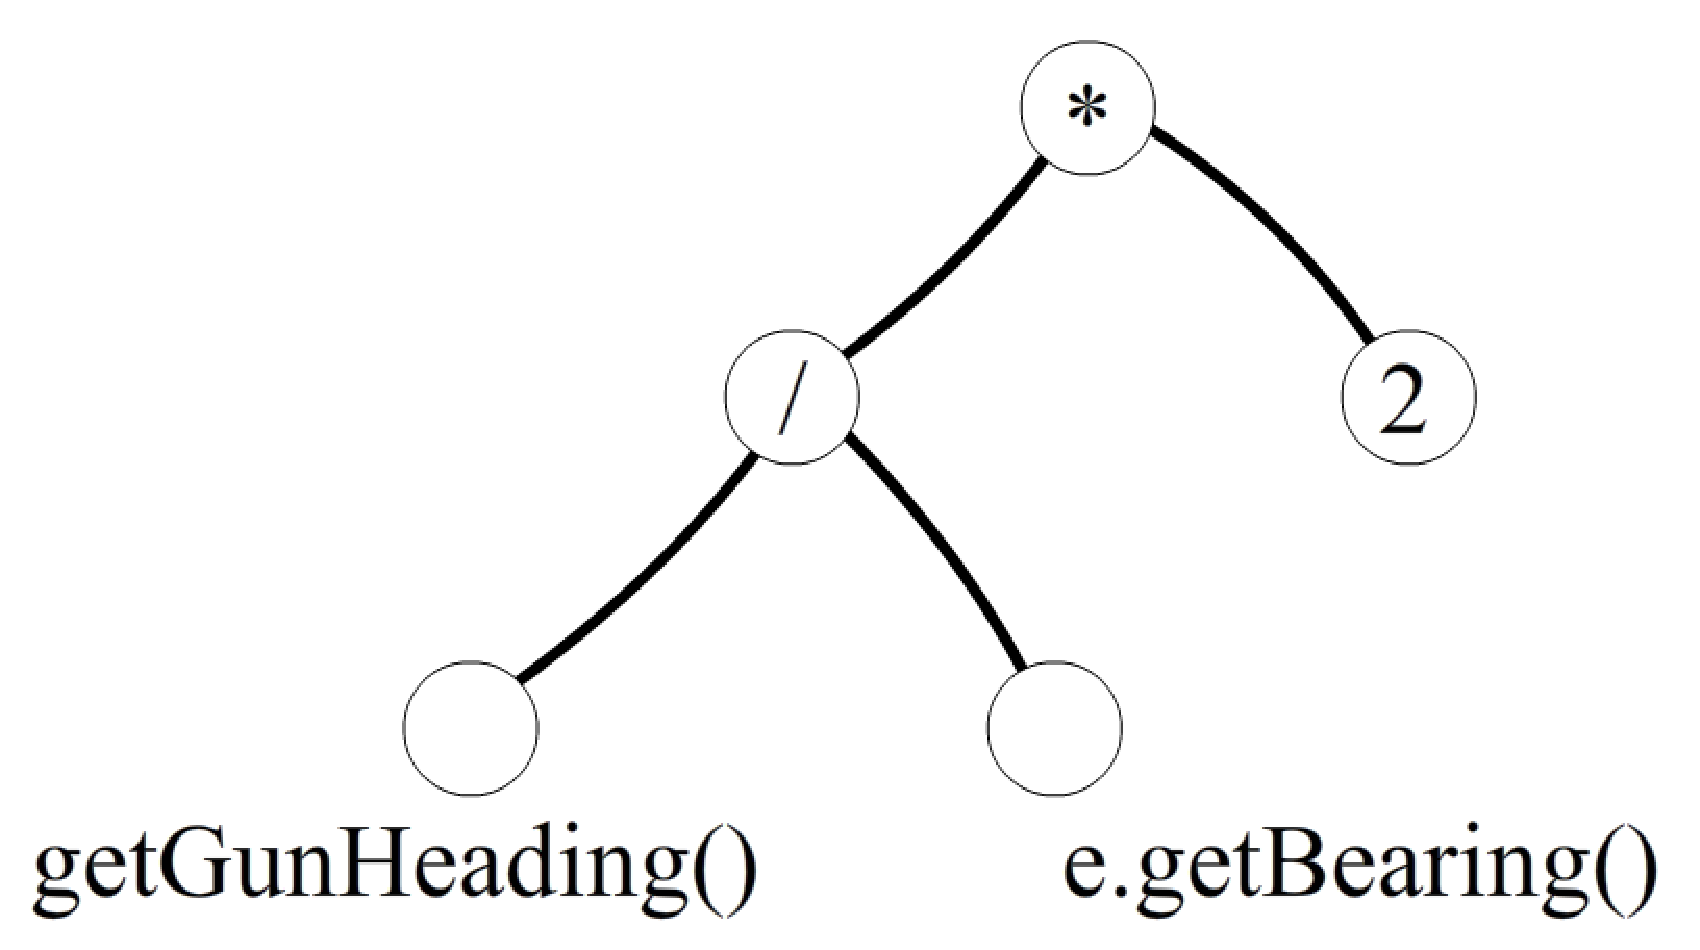
\includegraphics[scale=0.2]{tree}
    \caption{An expression tree.}
    \label{fig:tree1}
\end{figure}     

The second datastructure was needed because we value the potential of our program to evolve impressive 
mathematical functions highly. An \textit{ExpressionTree} is a binary tree holding both operators and 
values. Figure \ref{fig:tree1} shows the expression tree that represents equation \ref{eq:tree2}. 
This representation allows us to easily mutate expressions. To add, remove or alter a node 
one only has to recursively walk down a tree to the preferred node or leaf that needs to be altered.  

\begin{equation}
    \frac{getGunHeading()}{e.getBearing()}*2
    \label{eq:tree2}
\end{equation}

These datastructures are implemented in \textit{AESIGene}. We have decided that each relevant event such as \textit{onHitByBullet} or \textit{onHitWall} can be filled with Java code so each such an event represents a gene. Genes are filled with the previously mentioned datastructures and are mutated during evolution. Representing information on such a gene is currently not yet implemented but should be so in the future when we need to safe data in order to benchmark. 
 
\subsection{Phenotype}
The phenome is the resulting behaviour of the bot. Currently no real powerful behaviour has been generated. This is because not every important aspect is implemented. More of this can be found in the section \textit{result}.

\subsection{Meta language}
We need to design a meta language that creates java code from a genetic code. The genetic code is a string of digits, the location of the digit tells what gene is described, the value describes what this specific gene does. It is important to keep the genetic code meaningful and understandable so we can use the genetic code to ``see'' what kind of behaviour is evolved. This prevents our evolutional process to become a black box we use to evolve bots but where it is hard to really understand what is going on.

To properly describe how this works, we will show how java code of a simple bot, provided by RoboCode, can be represented in our genes.
This is the code of the simple bot:
\lstinputlisting[language=Java]{SpinBot.java}

This code can be described in a tree, like this:\\

\synttree[ SpinBot [ Run [ setTurnRight(10000) ] [ setMaxVelocity(5) ] [ ahead(10000) ] ] [ onScannedRobot [ fire(3) ] ] [ onHitRobot [ {if(...)} [ turnRight(10) ] ] [ isMyFault() ] ] ]

The computer will see the tree like this:\\

\synttree[ 0 [ 0 [ 12(10000) ] [ 13(5) ] [ 10(10000) ] ] [ 1 [ 3(3) ] ] [ 2 [ \#if [ 12(10) ] ] [ 4  ] ] ]

Here the upper number is an index of the gene, and the numbers on the second row are numbers indicating the index of the gene array. Under that we have array indices of the methods and their arguments, that are positioned in arrays with all the methods we can call and the arguments we can give them.


\subsection{Fitness function}
Fitness is crucial to determining the trajectory of the evolutionary process. Based on the fitness score, the program decides which chromosomes are transferred to the next generation of bots.

With the fitness function, we translate battle results into a appropriate fitness value. Our basic scoring measure is the fractional score F, which is computed using the score gained by our bot $S_b$ and the score gained by its adversary $S_a$.

Calculating the fitness score this way, we encourage our bot not only to maximize its own score, but to do so at the expense of its enemy.

\begin{eqnarray*}
	& F = 100 \times (1 + \frac{S_p - S_a}{S_p + S_a})\\
	& \mbox{Equation \theequation\addtocounter{equation}{1}. The fitness function.}
\end{eqnarray*}

In early stages of the evolutionary process, bots obtain no points at all. To prevent the program dividing with zero we created a catch in the code. If both scores are zero, both bots will be given a zero as fitness value.

\subsection{Evolve}
Because we still need to finish some major functions we have not started evolving as of yet. We do have some results which can be found in the section \textit{results}. 

\section{Results}
Currently our program has evolved a single bot, which is capable of doing something. The results are, as discussed in previous sections, minimal, but prove promising. The robot shows action such as moving forward and rotating both it's body and gun but not yet a change in behaviour when events are caught. This means we completed the basis but need to focus on the evolutionary process that will create bots with more interesting behaviour.

We need to be able to compare our results to other bots to give the results a meaning. During this project we will create some bots ourselves and download bots that have proven to be powerfull in online tournaments. These bots will be battling against our bots. This way we can find out if the bots evolved with genetic programming can stand against human made bots. There is a paper ``GP-Robocode: Using Genetic Programming to Evolve Robocode Players'' \cite{shichel} about RoboCode bots evolved with a genetic framework that participated in a online tournament with 27 participants. Other bots were all human written. The bot (``GPBot'') ended third.

\section{Problems}
\label{sec:problems}
\subsection{JGAP Framework}
Our decision to program in the JGAP Framework has turned out to be quite a bad one. Besides the days of effort we put into setting up JGAP we also lost a lot of time attempting to get JGAP to work. Of course JGAP did something but not at all what we wanted it to do or what we expected.\\

JGAP uses a \textit{Configuration} object in which it stores, among others the \textit{Fitness Function} object and the \textit{Population}. But also settings and other configurations. This is immidiately confusing as we do not have an idea what these settings are or what how the population is build up. We also had to implement functions we had no need for and had to use with variables (arguments) we did not want. This was easily handled as we did not use what we did not need but when the results started to role in we were baffled.\\

These results were very dissapointing. Our bots did evolved, but they did not get any high fitness values. We found out that after a few hunderds of rounds the bots devolved, bringing us back where we started.\\
We first thought this was because our fitness function was incorrect. We updated the function but this did not change the results.\\
We then did a lot of simulations to test our parameters. Using a different population size and different amount of battles to calculate the fitness value did have influence, but did not solve the devolution.\\

Our next hypothesis was that settings within the JGAP Framework might be the cause for the unexpected reults. After we had did some serious internet research and code inspectations we had to conclude that we could not figure out how JGAP exactly works. The framework is quite big, but its options are not adequately documented.\\

To demonstrate our troubles with this framework, we describe the \textit{Natural Selector} object and its implementation by JGAP might demonstrate our troubles with this framework. At one point in time we tried to simply safe the chromosomes with a high fitness value. We needed to create an object and add it to the \textit{Configuration} object. One would think this is not a problem but JGAP stores these \textit{Natural Selectors} in an ordered chain of registered selectors. The \textit{Configuration} object can also be locked and not be unlocked once it is unlocked. And lastly, the \textit{Configuration} object sometimes resets data to \textit{null}. Once we took care of all these problems we could start testing, but this took a lot time and results were inconclusive.\\

A short summary of our problems with JGAP.

\begin{enumerate}
    \item Learning to set up the framework and basic functioning. JAR files, buildpaths, classpaths, Eclipse. It's all very confusing.
    \item The JGAP Framework worked like a black box. With only a known input and output, it is difficult to locate problems inside the program. 
    \item Bad and incomplete documentation. A function needs input, but what format is this input? What does this function even do? These are only two examples of many problems we had with JGAP and where the documentation did not help us at all.
    \item Unnecessary functions. Our design for the evolutional process is quite simple and elegant. We found that using complicated JGAP code, these simple things turned out to be very difficult. For example, if we want to select the 10 fittest chromosomes of our population we had to go through a chain of registred selectors or find out how or why the configuration is locked or reset.
    \item Dismissable results. De-evolving at times without any reason.
    \item Unexpected behaviour. Some poorly chosen engineering decisions result in forced use of classes we known nothing about. For example \textit{IChromosome}, because this is an interface, it has certain restrictions. We wanted to store addiontal information in such a class, for example a method to create code from a chromosome. This is not possible in an interface. JGAP works around this problem with a slot for the ApplicationData, which can be any object. This is object is however sometimes, seemingly randomly reset to \textit{null}.
\end{enumerate}

\subsection{Leaving JGAP Framework Behind}
With more and more experience with genetic programming, it became more and more clear that we did not need such a complicated framework. In one afternoon a simple framework was written that did exactly what we wanted. Another afternoon was used to rewrite the code into something more structured using an OOP approach. Now, with extremely well-ordered and structured code we could start running more definitive simulations, debug and expand the potential capabilities of our robots.\\

Because we were not sure if it was just JGAP or JGAPs settings that were responsible for the previously achieved horrible results we made sure the top performing chromosomes always survived by implementing algorithm \ref{alg:main}.

\begin{algorithm}
\begin{algorithmic}
\STATE Initialize Population
\WHILE{true}
    \STATE Evolve Bottom 50\%
    \STATE Evaluate Bottom 50\%
    \STATE Sort Population 
    \STATE Replace Bottom 50\% With Top 50\%
\ENDWHILE
\end{algorithmic}
\caption{Main Evolution Algorithm}
\label{alg:main}
\end{algorithm}

After the first simulations it became clear that the evolutionary process was not going as expected. While the robots did not seem to devolve, new or mutated chromosomes did not seem to have any improvements. New generations had similar fitness values, but sometimes there was a very big decrease or increase in the fitness value.\\
This happened even though new chromosomes should be only slightly different from the other chromosomes. Even with our newly gained debug capabilities and advantages of not using JGAP but our own code we could not figure out what was causing these results.\\
For further testing purposses we created a graphical representation of the fitness values throughout the evolution process so we can easily find out when in time what fitness value were achieved. This helped u a lot, especially while debugging or evaluating performance of various parameters.\\

We plot the following three values: the biggest fitness value in red, the average fitness value of the total population in blue and the average fitness value of the newly mutated chromosomes in a population in green. The first results, shown in figure \ref{fig:result_1} clearly explain what is going on.\\

\begin{figure}[h!]
  \centering
  \subfloat[3.7 After 7 rounds ]{\label{fig:result_1_1}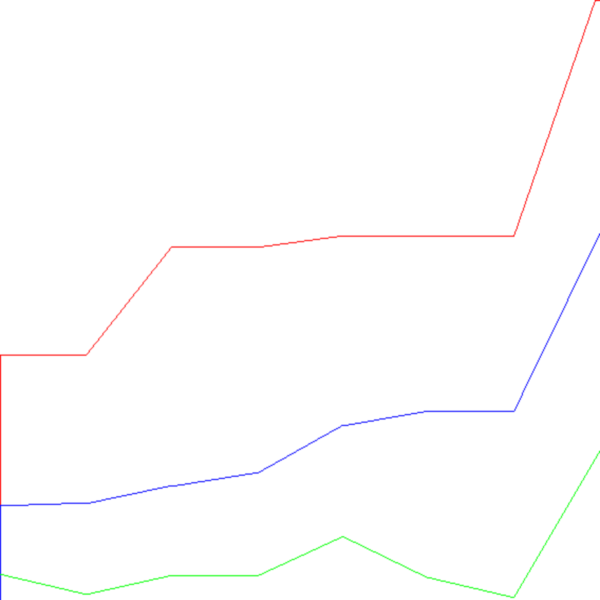
\includegraphics[width=0.3\textwidth]{result_1_1}}
  \subfloat[9.5 After 33 rounds]{\label{fig:result_1_2}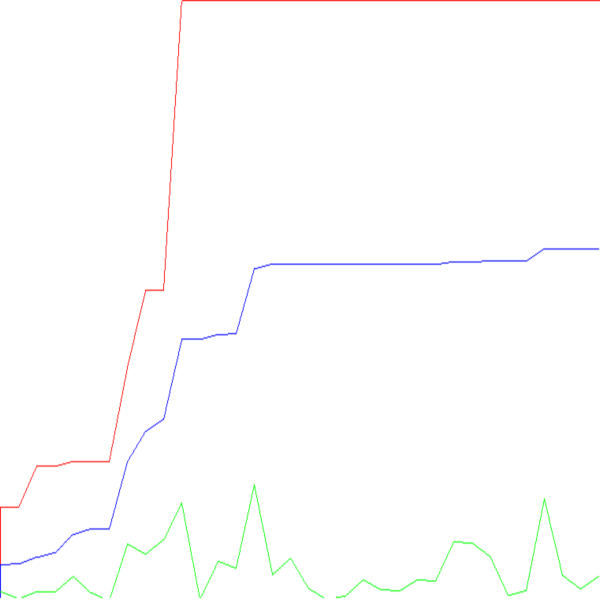
\includegraphics[width=0.3\textwidth]{result_1_2}}
  \subfloat[35 After 65 rounds]{\label{fig:result_1_3}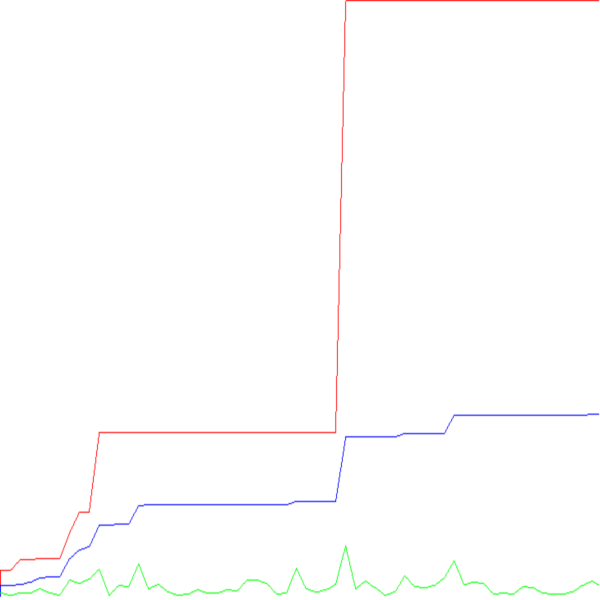
\includegraphics[width=0.3\textwidth]{result_1_3}}
  \caption{Graphical representation of fitness values throughout generations at different times}
  \label{fig:result_1}
\end{figure}

The results clearly show that the highest fitness value remains in the population. It also indicates that the top fitness values remain in the population as the average does not decrease. However, the average of newly mutated chromosomes is always dissapointingly low. This was thought to be extremely unlikely as one simple mutation should not have such a major impact on the whole generation causing the fitness value drops to zero. In the mean time, the best robots showed promising results!\\

For a while we had no idea what was going on. When we discovered that sometimes the best robot the program wrote to a file wasn't actually the best robot in the program that we build in a check that reevalutes the complete population every 10 evolution rounds. The result is shown in figure \ref{fig:result_2}.

\begin{figure}[h!]
    \centering
    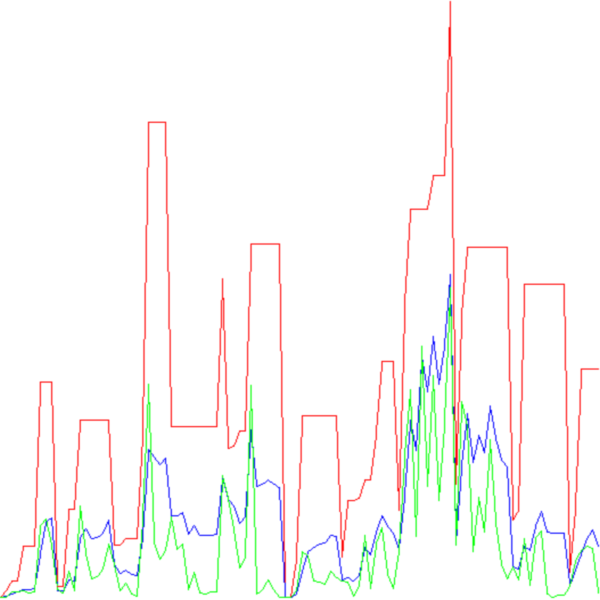
\includegraphics[width=0.5\textwidth]{result_2}
    \caption{The results with a reevaluation every 10 rounds}
    \label{fig:result_2}
\end{figure}

It seemed the fitness value was constant but the chromosomes continued to evolve. After examining our algorithm even further we were still unable to find any bugs.\\
When we almost gave up we remembered how Java does not always stores a copy of an object but actually a copy of the reference to the object. This would explain everything and with the Java/Eclipse debugger we could validate this. The easy fix was to clone our chromosomes.\\

The first results proved promising but still not what we expected. After more research we learned we had to clone every object, and not just the chromosomes. Our program stores objects in objects using arrays. We assumed incorrectly cloning the first layer (chromosome) would be sufficient, instead we had to clone up untill the deepest stored objects in our program. Every layer (see figure \ref{fig:layers}) of our program had to be cloned in a specific manner. It took us a lot of time to figure out that this actually had to be done for each layer. Especially the last layer, the \textit{ExpressionTree} which is recursively stored was tricky.\\

\begin{figure}[h!]
    \centering
    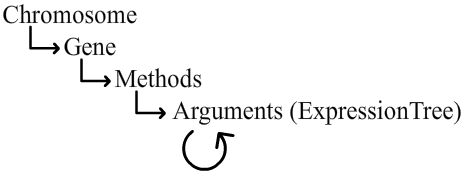
\includegraphics[width=0.5\textwidth]{layers}
    \caption{The depth of our program depends on the depth of an \textit{ExpressionTree}}
    \label{fig:layers}
\end{figure} 

After this ephiphany implementation was easy and we could finally start evolving. As we had expected in the beginning, robots did not devolve and when they did only minimally. The results in figure \ref{fig:result_3} clearly shows a rising average fitness value! The ninetieth generation was able to deliver robots that could beat our default opponent \textit{Spinbot}. We were very happy with this!

\begin{figure}[h!]
  \centering
  \subfloat[41 After 41 rounds]{\label{fig:result_3_1}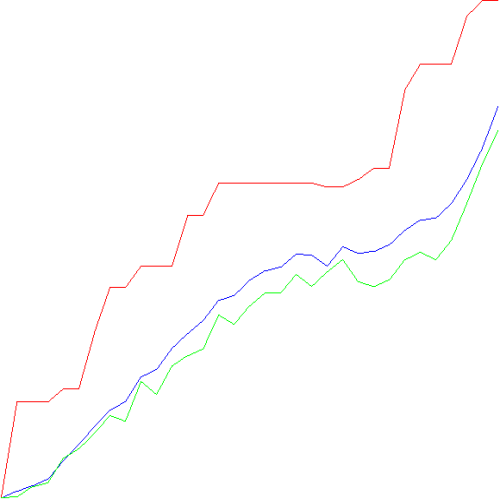
\includegraphics[width=0.4\textwidth]{result_3_1}}
  \subfloat[120 After 102 rounds]{\label{fig:result_3_2}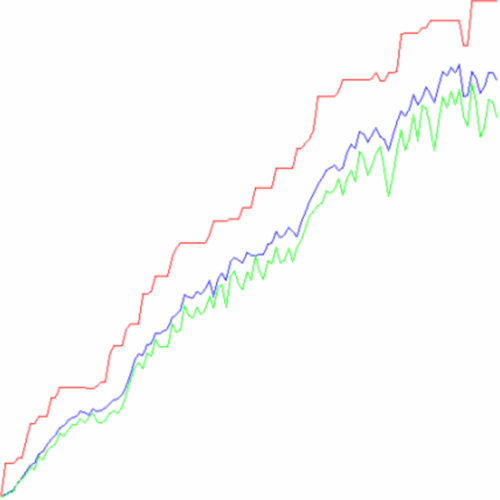
\includegraphics[width=0.4\textwidth]{result_3_2}}
  \caption{Graphical representation of fitness values throughout generations at different times showing correct results.}
  \label{fig:result_3}
\end{figure}

\subsection{Creating our own Framework, a Good Decision?}
Creating our own framework definitely helped us find, identify and solve the problems. Our well structured code now allows us to easily change parameters and even the basic functioning of the program. However, we currently do not know if the unexpected results produced by JGAP were produced by the same kind of programming mistakes. If this is the case some of the problems might not have been caused by JGAP.\\

While it is easy to change the parameters and basic functioning of the program, changing something more advanced such as the manner on which the program selects the best genes costs significantly more time. Perhaps even more time in our framework then in it would have had in JGAPs.\\
For example, there are multiple efficient methods to gather information. The robot could scan the entire room by turning the radar continuously or the robot could keep the radar fixed on the target. It is generally accepted that the latter method results in a higher fitness value.
However, bots in earlier generations cannot have such complicated behaviour and will almost always perform simple scan behaviour that evolves into a less powerfull scan method. Once a bot has a certain method for scanning, it is almost impossible to evolve the different, better method as there are multiple evolution cycles needed to evolve to the different information gathering method. In the mean time, while evolving, it has no information gathering method making it extremely unlikely that the robot achieves an high enough fitness value to survive and evolve further.\\

There are two things that could fix this. We could select the genes that survive based on their fitness value and a chance or we could implement cross mutation.

\section{Background information}
\label{bi}
\subsection{RoboCode Game}
Time is represented in ticks. There are several things happening each tick. For example the robot is allowed a certain amount of processing time to calculate and execute actions. The game world is also updated, meaning that objects are relocated according to the physical laws of the game and potential collisions between objects and the results of such collisions are calculated.

\subsection{Robot Anatomy}
A robot consists of three seperate parts, the radar which is mounted on the barrel which is mounted on the body. All parts can be rotated seperately. The barrel fires bullets, the radar scans for other tanks and the body drives around in the arena.

\begin{figure}[h!]
    \centering
    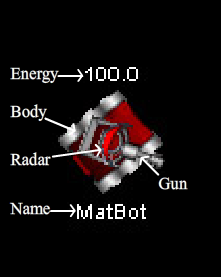
\includegraphics[width=0.25\textwidth]{botatom}
    \caption{The anatomy of a RoboCode bot}
\end{figure} 

\subsection{Robocode rules}
The Robocode environment has specific rules constraining our bot. A fight starts by placing all participating bots in the arena at random places. All bots have a certain amount of energy. Energy is lost by getting shot by an enemy or ramming walls and enemies. Certain actions also use up energy, for example shooting a bullet.
A bot can gain energy by hitting an opponent.
When a bot is out of energy, it is disabled and explodes when hit by a bullet.

\subsection{Programming the Robot}
Programming a robot means \textit{extending} a certain robot class from RoboCode, we use Advanced-Robot. This allows us to program methods that catch events that are launched by RoboCode (such as \textit{robotScannedEvent}, this event is launched when a bot scans another bot) and program what we would like the robot to do in such cases (such as \textit{rotateGun}, this method rotates the barrel changing the direction of a fired bullet). The robots behavior relies completely on what events occur during a battle. The robots actions during a certain event is generated by the evolutionary process.

\newpage
\section{Planning}
\subsection{Documentation}
\begin{itemize}
 \item create workplan, everybody
 \item round of halfway report and presentation, M. de Waard
 \item present halfway presentation, everybody
 \item finish end report and presentation, J. Rooijmans
 \item present final product, everybody
 \item maintain documentation, M. Inja
\end{itemize}

\subsection{Initiation}
\begin{itemize}
\item create planning and set up websites, M. Inja
\item present workplan, everybody
\item familarization with programs, M. Inja, M. de Waard
\item read articles about genetic algoritms, J. Rooijmans
\end{itemize}

\subsection{Genetic programming, single bots}
\begin{itemize}
\item create genotype, J. Rooijmans
\item create fitness function, M. de Waard
\item evolve, M. Inja
\end{itemize}

\subsection{Test phase}
\begin{itemize}
\item benchmark with RoboResearch, M. de Waard
\item compare RoboCode with JPAG, M. Inja
\item design and compare with own bot, everybody
\item compare with bots from the internet, J. Rooijmans
\end{itemize}

\subsection{Genetic programming, teams}
\begin{itemize}
\item create genotype, J. Rooijmans
\item create fitness function, M. de Waard
\item evolve, M. Inja
\item benchmark, everybody
\end{itemize}
\newpage
\bibliographystyle{abbrv}
\bibliography{ref}
\newpage
\appendix
\section{Planning}
\label{planning}
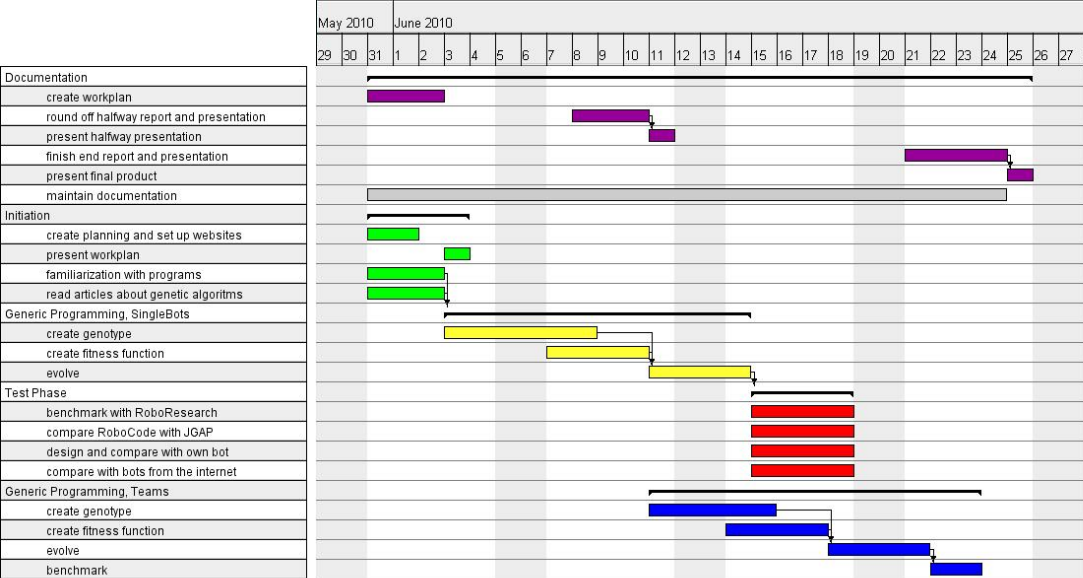
\includegraphics[height=0.75\textwidth, angle=-90]{planning.png}
\end{document}
